\section{Efficiency}
\label{sec:Lb_eff}

The selection efficiency is calculated for each decay according to the formula
%\begin{equation}
%\label{eq:Lmumu_eff}
%\varepsilon^{tot}=\varepsilon(Geom)\,\varepsilon(Det|Geom)\,\varepsilon(Reco|Det)\,\varepsilon(MVA|Reco)\,\varepsilon(Trig|MVA).
%\end{equation}
\begin{equation}
\label{eq:Lmumu_eff}
\varepsilon^{tot} = \varepsilon^{\rm geom} \cdot \varepsilon^{\rm det|geom} \cdot \varepsilon^{\rm reco|det} \cdot \varepsilon^{\rm MVA|reco} \cdot \varepsilon^{\rm trig|MVA}
\end{equation}
In this expression the first term represents the geometric efficiency, \emph{i.e.} the fraction of events where
the muons of the decay candidate are inside the LHCb acceptance.
The second term handles the possibility of the \Lz either escaping the detector or interacting with it and therefore
never decaying into $p\pi$; this term is referred to as ``detection" efficiency.
The third term carries information about the reconstruction and pre-selection efficiencies,
which are considered together given that boundaries between them are arbitrary.
The fourth part describes the efficiency of the neural network for candidates that have passed the pre-selection criteria. 
Finally, the last term handles the trigger efficiency for candidates which are accepted by the full selection.
%Trigger efficiency is calculated before the MVA one because the training is performed on untriggered data to save statistics.
Most of the efficiency components are evaluated using the simulated samples described in Sec.~\ref{sec:Lb_simulation}.
The efficiency of the PID requirement for the proton (see Tab.~\ref{tab:Lb_stripping}) is derived separately 
using a data-driven method because the simulation does not provide a good description of PID variables. 
%For complete information, all absolute efficiencies for the two decays $\Lb\to\Lz\mumu$ and $\Lb\to\jpsi\Lz$ are
%separately listed in the next subsections. 
Although the analysis itself only depends on the relative efficiency,
$\varepsilon(\Lb\to\Lz\mumu)/\varepsilon(\Lb\to\jpsi\Lz)$, representative values of the absolute efficiencies 
for each of the five terms in Eq.~\ref{eq:Lmumu_eff} are given in the following sections for completeness.. 


\subsection{Geometric acceptance}
\label{sec:Lb_geomAcc}
In order to save disk space and time the simulation only includes events in which the final muons
are inside the detector acceptance and therefore can be reconstructed. This corresponds to a requirement for each
of the muons to be in an interval \mbox{$10 < \theta < 400$~mrad}, where $\theta$ is the angle between
the muon momentum and the beam line. The efficiency of this requirement is obtained by using 
a separate simulated sample, where events are generated in the full $4\pi$ solid angle.
The geometric efficiency varies between 18\% at high-\qsq and 20\% at low-\qsq;
Fig.~\ref{fig:Lb_absEff} shows the dependence of this efficiency as a function of \qsq.

%In Tab.~\ref{tab:Lb_geom_eff} the efficiencies due to the geometrical acceptance are listed
%in bins of \qsq for $\Lb\to\Lz\mumu$ decays.
%
%\begin{table}[h]
%\centering
%\caption{Absolute geometrical acceptance in the two integrated \qsq bins
%derived from generator level simulated samples. Uncertainties are statistical only.}
%\begin{tabular}{$l^c}
%\rowstyle{\bfseries}
%\boldmath{\qsq} [\boldmath{\gevgevcccc}]     & \boldmath{$\varepsilon(Geom)$}   \\ \hline
%0.1--2.0 		&  $0.2359 \pm 0.0008$  \\
%2.0--4.0 		&  $0.2098 \pm 0.0007$  \\
%4.0--6.0 		&  $0.2008 \pm 0.0007$  \\
%6.0--8.0 		&  $0.1960 \pm 0.0008$  \\
%9.1--10.1 	&  $0.1927 \pm 0.0012$  \\
%11.0--12.5 	&  $0.1897 \pm 0.0010$  \\
%15.0--16.0 	&  $0.1896 \pm 0.0015$  \\
%16.0--18.0 	&  $0.1872 \pm 0.0012$  \\
%18.0--20.0 	&  $0.1870 \pm 0.0016$  \\
%\hline
%\phantom{x}1.1 -- 6.0\phantom{x} 	&  $0.2072 \pm 0.0005$  \\
%15.0 -- 20.0 	&  $0.1876 \pm 0.0008$  \\
%\end{tabular}
%\label{tab:Lb_geom_eff}
%\end{table}


\subsection{Reconstruction and neural network efficiencies}

The efficiency to reconstruct the decays together with the pre-selection requirements is
evaluated from simulated data. 
%For the evaluation we use the most recent LHCb measurement of \Lb
%lifetime of $1.482\pm0.03$ ps\cite{LHCb--PAPER--2013--032} and \Lb polarisation $0.06\pm0.09$ \cite{Aaij:2013oxa}.
%Table~\ref{tab:Lb_recoEff} reports values of reconstruction efficiency for the two integrated \qsq intervals
 %for long and downstream candidates.
The reconstruction efficiency is subdivided in ``Detection" and ``Reconstruction and pre-selection" efficiencies.
In fact, since the \Lz is a long lived particle, there is a non-negligible probability for it to interact with the detector
or escape from it; in these cases it cannot be detected as a proton and a pion. 
%The efficiency for this to happen is what is called ``Detection" efficiency. 
The reconstruction efficiency includes the probability 
for the tracks to produce observable signatures and to pass the pre-selection 
requirements. This component does not include the efficiency
of the PID cut that appears in Tab.~\ref{tab:Lb_stripping}, which is kept separate
because PID variables are not well described by the simulation.
The detection efficiency varies between 88\% at low-\qsq and 92\% at high-\qsq
while the reconstruction efficiency is almost flat in \qsq at 6.6\% for downstream candidates
and 2.0\% for long candidates.
%Fig.~\ref{fig:Lb_absEff} shows the dependence of these efficiencies as a function of \qsq.
% and therefore a data-driven method is used instead (see Sec.~\ref{sec:PIDeff}).
%
%
%\begin{table}[h]
%\centering
%\caption{Absolute detection and reconstruction plus stripping efficiencies.
%Reconstruction efficiency is given separately for downstream and long candidates. Uncertainties are statistical only. }
%\begin{tabular}{$l^c^c^c}
%\rowstyle{\bfseries}
%\boldmath{\qsq} [\boldmath{\gevgevcccc}] & \boldmath{$\varepsilon(Det)$} & \boldmath{$\varepsilon(Reco)^{\rm DD}$} & \boldmath{$\varepsilon(Reco)^{\rm LL}$} \\ \hline
%0.1--2.0 		&  $0.8793 \pm 0.0005$	&  $0.0519 \pm 0.0006$	&  $0.0194 \pm 0.0004$  \\
%2.0--4.0 		&  $0.8850 \pm 0.0004$	&  $0.0664 \pm 0.0006$	&  $0.0195 \pm 0.0004$  \\
%4.0--6.0 		&  $0.8902 \pm 0.0004$	&  $0.0717 \pm 0.0007$	&  $0.0209 \pm 0.0004$  \\
%6.0--8.0 		&  $0.8962 \pm 0.0005$	&  $0.0756 \pm 0.0007$	&  $0.0212 \pm 0.0004$  \\
%9.1--10.1 	&  $0.9022 \pm 0.0007$	&  $0.0787 \pm 0.0011$	&  $0.0220 \pm 0.0006$  \\
%11.0--12.5 	&  $0.9084 \pm 0.0006$	&  $0.0799 \pm 0.0009$	&  $0.0221 \pm 0.0005$  \\
%15.0--16.0 	&  $0.9187 \pm 0.0009$	&  $0.0736 \pm 0.0012$	&  $0.0179 \pm 0.0007$  \\
%16.0--18.0 	&  $0.9247 \pm 0.0007$	&  $0.0696 \pm 0.0010$	&  $0.0169 \pm 0.0005$  \\
%18.0--20.0 	&  $0.9318 \pm 0.0009$	&  $0.0600 \pm 0.0011$	&  $0.0136 \pm 0.0006$  \\
%\hline
%\phantom{x}1.1 -- 6.0\phantom{x} 	&  $0.8868 \pm 0.0003$	&  $0.0684 \pm 0.00041$	&  $0.0202 \pm 0.0002$  \\
%15.0 -- 20.0 	&  $0.9260 \pm 0.0005$	&  $0.0669 \pm 0.00063$	&  $0.0159 \pm 0.0003$  \\
%\end{tabular}
%\label{tab:Lb_recoEff}
%\end{table}
%
%\subsubsection{Neural Networks efficiency}
%
The MVA selection efficiency is again evaluated from simulated samples
and it is observed to vary between 55\% and 88\% for downstream candidates
and between 74\% and 96\% for long candidates.
Figure~\ref{fig:Lb_absEff} shows the dependence of these efficiencies as a function of \qsq.
%Results are shown in 
%Tab.~\ref{tab:Lb_mvaEff} for the two integrated \qsq intervals.
The sudden jump in MVA efficiency at $\sim 9$~\gevcc~is due to the fact that
a different figure-of-merit is used to optimise the MVA requirement in the low- and high-\qsq regions,
which results in different efficiencies.
%
%\begin{table}[h]
%\centering
%\caption{Neural network selection efficiency. Uncertainties are statistical only.}
%\begin{tabular}{$l^c^c}
%\rowstyle{\bfseries}
%\boldmath{\qsq} [\boldmath{\gevgevcccc}] & \boldmath{$\varepsilon(MVA)^{\rm DD}$} & \boldmath{$\varepsilon(MVA)^{\rm LL}$}\\ \hline
%0.1--2.0 		&  $0.623 \pm 0.008$	&  $0.813 \pm 0.011$  \\
%2.0--4.0 		&  $0.583 \pm 0.007$	&  $0.757 \pm 0.011$  \\
%4.0--6.0 		&  $0.584 \pm 0.007$	&  $0.776 \pm 0.011$  \\
%6.0--8.0 		&  $0.588 \pm 0.007$	&  $0.778 \pm 0.011$  \\
%9.1--10.1 	&  $0.904 \pm 0.006$	&  $0.948 \pm 0.008$  \\
%11.0--12.5 	&  $0.888 \pm 0.005$	&  $0.944 \pm 0.007$  \\
%15.0--16.0 	&  $0.882 \pm 0.007$	&  $0.929 \pm 0.012$  \\
%16.0--18.0 	&  $0.847 \pm 0.007$	&  $0.928 \pm 0.009$  \\
%18.0--20.0 	&  $0.831 \pm 0.009$	&  $0.889 \pm 0.016$  \\
%\hline
%\phantom{x}1.1 -- 6.0\phantom{x} 	&  $0.584 \pm 0.005$	&  $0.772 \pm 0.007$  \\
%15.0 -- 20.0 	&  $0.849 \pm 0.005$	&  $0.917 \pm 0.007$  \\
%\end{tabular}
%\label{tab:Lb_mvaEff}
%\end{table}

%This efficiency component was crosschecked using \jpsi real data. In these events the peak is well visible even before
%the MVA cut. Therefore it is possible to fit the peak to subtract the background and then do the same procedure after the MVA cut.
%Counting events in an interval of 20 $MeV/c^2$ around the \jpsi invariant mass and (5605,5635) in \Lb invariant mass
%we obtain the following efficiencies: 86.1\% for DD events and 93.1\% for LL.
%Given the uncertainty on the background subtraction prodecure we quintify the uncertainty on this procedure
%in $\sim 4\%$ by varing mass windows and look at the change in the efficiency obtained. The pure statistical error
%on these values is 0.7\%. Therefore comparing numbers in table \ref{tab:jpsiEff}, obtained using \jpsi\Lz MC, we find them compatible within 1 sigma.   



\subsection{Trigger efficiency}
\label{sec:Lb_trigger_eff}

The trigger efficiency is also evaluated using a simulated sample. It increases with \qsq and varies 
from $\sim 57\%$ to $\sim 86\%$ for both downstream and long candidates.
Figure~\ref{fig:Lb_absEff} shows the dependence of this efficiency as a function of \qsq.
To increase confidence in these evaluations, 
%Using the high statistics resonant channel it is possible to crosscheck using data 
the trigger efficiency obtained using the simulation is validated using data recorded in the high statistics resonant channel.
In LHCb triggered events can fall into two categories: those triggered by a track that is part of a signal candidate, 
Trigger On Signal (TOS), and those triggered by other tracks in the event that are not part of the signal candidate, 
Trigger Independent of Signal (TIS). As the TIS and TOS categories are not exclusive the TIS sample provides a control
sample which can be used to obtain the efficiency for TOS triggers. This can be calculated with the formula:
\begin{equation}
\varepsilon_{\rm TOS} = \frac{\text{TIS  and TOS }}{\text{TIS}}.
\end{equation}
As data contains background the numbers of signal candidates in the ``TIS" and \mbox{``TIS and TOS"}
categories are not just determined by counting but from fits to the 4-body invariant mass, 
$m(p\pi\mu\mu)$, distributions after applying these requirements. This procedure is referred to as the TISTOS method. 
Using this data-driven method an efficiency of ($70 \pm 5$)\% is obtained. This is consistent with, and hence validates, 
the significantly more precise value of ($73.33 \pm 0.02$)\% obtained using the simulation.
%
%\begin{table}[h]
%\centering
%\caption{Absolute trigger efficiencies for selected events as determined
%from the simulation separately for downstream and long events.}
%\begin{tabular}{$l^c^c} 
%\rowstyle{\bfseries}
%\boldmath{\qsq} [\boldmath{\gevgevcccc}] & \boldmath{$\varepsilon(Trig)^{\rm DD}$} & \boldmath{$\varepsilon(Trig)^{\rm LL}$}\\ \hline

%0.1--2.0 	&  $0.560 \pm 0.008$	&  $0.577 \pm 0.012$  \\
%2.0--4.0 	&  $0.606 \pm 0.006$	&  $0.651 \pm 0.010$  \\
%4.0--6.0 	&  $0.623 \pm 0.006$	&  $0.674 \pm 0.010$  \\
%6.0--8.0 	&  $0.669 \pm 0.006$	&  $0.706 \pm 0.010$  \\
%9.1--10.1 	&  $0.700 \pm 0.007$	&  $0.722 \pm 0.013$  \\
%11.0--12.5 	&  $0.744 \pm 0.006$	&  $0.738 \pm 0.011$  \\
%15.0--16.0 	&  $0.818 \pm 0.008$	&  $0.826 \pm 0.015$  \\
%16.0--18.0 	&  $0.836 \pm 0.006$	&  $0.860 \pm 0.011$  \\
%18.0--20.0 	&  $0.857 \pm 0.008$	&  $0.863 \pm 0.015$  \\
%\hline
%\phantom{x}1.1 -- 6.0\phantom{x} 	&  $0.610 \pm 0.004$	&  $0.653 \pm 0.007$  \\
%15.0 -- 20.0 	&  $0.839 \pm 0.004$	&  $0.853 \pm 0.008$  \\
%\end{tabular}
%\label{tab:Lb_triggerEfficiency}
%\end{table}


\subsection{PID efficiency}
\label{sec:PIDeff}
For long tracks a PID requirement on protons (\verb!PID!p$ > -5$) is applied. The simulation is known not to
describe PID variables well and therefore a data-driven method is used to obtain this efficiency component.
This is done using the \verb!PIDCalib! package (see Sec.~\ref{sec:PID_calib}), which uses samples of
decays where particles can be identified due to their kinematic properties as calibration samples. In the case of protons 
a sample of \Lz particles is used, where the proton can be identified because it always has the highest momentum.
The package allows the phase space to be divided into bins of variables relevant for PID
performances; in this analysis, momentum and pseudorapidity are used.
Using the calibration sample the efficiency is derived in each two-dimensional bin.
Finally, to take into account the possibility that the decay channel under study could have different kinematical distributions
than the calibration sample, these efficiency tables are used to re-weight the simulation.
The PID efficiency varies from 97.3\% at low-\qsq to 98.2\% at high-\qsq. 
%Absolute PID efficiencies are listed in Tab.~\ref{tab:Lb_PIDabs} for the two integrated \qsq intervals.
%
%\begin{table}[h]
%\centering
%\caption{Absolute PID efficiencies in \qsq bins.}
%\begin{tabular}{$l^c}
%\rowstyle{\bfseries}
%\boldmath{\qsq} [\boldmath{\gevgevcccc}]	&      \boldmath{$\varepsilon(PID)$}  \\  \hline
%0.1--2.0     &  $97.32 \pm 0.012$   \\
%2.0--4.0     &  $97.42 \pm 0.012$   \\
%4.0--6.0     &  $97.59 \pm 0.011$   \\
%6.0--8.0     &  $97.70 \pm 0.010$   \\
%11.0--12.5   &  $98.04 \pm 0.009$   \\
%15.0--16.0   &  $98.31 \pm 0.006$   \\
%16.0--18.0   &  $98.10 \pm 0.005$   \\
%18.0--20.0   &  $98.11 \pm 0.001$  \\
%\hline
%\phantom{x}1.1 -- 6.0\phantom{x}     &  $97.49 \pm 0.007$   \\
%15.0 -- 20.0   &  $98.17 \pm 0.003$  \\
%\jpsi       &  $97.89 \pm 0.005$   \\
%\end{tabular}
%\label{tab:Lb_PIDabs}
%\end{table}



\subsection{Relative efficiencies}

In the previous sections absolute efficiency values were given for the rare channel, which are summarised in Fig.~\ref{fig:Lb_absEff}.
This section reports the corresponding relative efficiencies with respect to the $\Lb\to\jpsi\Lz$ channel, which will be
used to correct the yields and obtain the differential branching fraction. Table~\ref{tab:jpsiEff} reports the absolute 
efficiency values for the \jpsi channel used to derive the relative efficiencies.
Relative geometric, detection and PID efficiencies are listed in Tab.~\ref{tab:relativeGeometric}, while
Tabs.~\ref{tab:allRelativeEffDD} and \ref{tab:allRelativeEffLL} report relative reconstruction, trigger and MVA efficiencies 
separately for downstream and long candidates. Since the latter three components are obtained from the 
same simulated sample their statistical uncertainties are correlated. Therefore, the product of the three is also reported 
as a single efficiency and labeled ``Full Selection". Finally, Tab.~\ref{tab:Lb_effSummary} reports the overall relative efficiency, obtained 
as the product of all components, which will be then used to correct the raw yields and calculate the differential branching fraction.
Uncertainties reflect the statistics of both rare and resonant samples, while systematic uncertainties are discussed in following sections.

\begin{table}
\centering
\caption{Absolute efficiency values for $\Lb\to\jpsi\Lz$; uncertainties are statistical only.}
\begin{tabular}{$l^c^c}
\rowstyle{\bfseries}
Efficiency				& 	Downstream				& 	Long				\\  \hline		
$\varepsilon^{\rm geom}$ 	&   	\multicolumn{2}{c}{	$0.1818 \pm 0.0003$ } 	\\	
$\varepsilon^{\rm det}$ 	&   	\multicolumn{2}{c}{	$0.9017 \pm 0.0003$ } 	\\
$\varepsilon^{\rm reco}$	& 	$0.0724 \pm 0.0004$   & $0.0203 \pm 0.0002$     \\
$\varepsilon^{\rm pid}$	&	--	&  $97.89 \pm 0.005$   \\
$\varepsilon^{\rm MVA}$ 	&	$0.882 \pm 0.002$   & $0.942 \pm 0.002$     \\
$\varepsilon^{\rm trig}$ 	&	$0.697 \pm 0.003$   & $0.734 \pm 0.005$     \\ \hline
Full Selection			&	$0.0445 \pm 0.0003$   & $0.0140 \pm 0.0002$     \\ \hline
Total  				&	$0.00729 \pm 0.00005$   & $0.00230 \pm 0.00003$    	\\
\end{tabular}
\label{tab:jpsiEff}
\end{table}


\begin{table}
\centering
\caption{Relative geometric, detection and PID efficiencies between
$\Lb\to\Lz\mumu$ and $\Lb\to\jpsi\Lz$ decays; uncertainties reflect the statistics of both samples.}
\begin{tabular}{$l^c^c^c}
\rowstyle{\bfseries}
\boldmath{\qsq} [\boldmath{\gevgevcccc}] & Geometric & Detection & PID \\ \hline
%0.1--2.0 		&  $1.2976 \pm 0.0050$ 	&  $0.9751 \pm 0.0006$  \\
%2.0--4.0 		&  $1.1541 \pm 0.0043$ 	&  $0.9814 \pm 0.0005$  \\
%4.0--6.0 		&  $1.1043 \pm 0.0044$ 	&  $0.9872 \pm 0.0006$  \\
%6.0--8.0 		&  $1.0778 \pm 0.0045$ 	&  $0.9939 \pm 0.0006$  \\
%9.1--10.1 	&  $1.0596 \pm 0.0065$ 	&  $1.0005 \pm 0.0008$  \\
%11.0--12.5 	&  $1.0431 \pm 0.0058$ 	&  $1.0074 \pm 0.0007$  \\
%15.0--16.0 	&  $1.0426 \pm 0.0084$ 	&  $1.0188 \pm 0.0010$  \\
%16.0--18.0 	&  $1.0296 \pm 0.0068$ 	&  $1.0255 \pm 0.0008$  \\
%18.0--20.0 	&  $1.0288 \pm 0.0087$ 	&  $1.0333 \pm 0.0010$  \\
%\hline
%1.1 -- 6.0 	&  $1.1396 \pm 0.0031$ 	&  $0.9835 \pm 0.0004$  \\
%15.0 -- 20.0 	&  $1.0320 \pm 0.0048$ 	&  $1.0269 \pm 0.0006$  \\

\phantom{x}0.1 -- 2.0\phantom{x} 		&  $1.2976 \pm 0.0050$ 	&  $0.9751 \pm 0.0006$  & $0.99418 \pm 0.00013$ \\
\phantom{x}2.0 -- 4.0\phantom{x} 		&  $1.1541 \pm 0.0043$ 	&  $0.9814 \pm 0.0005$  & $0.99523 \pm 0.00013$ \\
\phantom{x}4.0 -- 6.0\phantom{x} 		&  $1.1043 \pm 0.0044$ 	&  $0.9872 \pm 0.0006$  & $0.99699 \pm 0.00012$  \\
\phantom{x}6.0 -- 8.0\phantom{x} 		&  $1.0778 \pm 0.0045$ 	&  $0.9939 \pm 0.0006$  & $0.99805 \pm 0.00011$ \\
11.0 -- 12.5 	&  $1.0431 \pm 0.0058$ 	&  $1.0074 \pm 0.0007$  & $1.00151 \pm 0.00010$ \\
15.0 -- 16.0 	&  $1.0426 \pm 0.0084$ 	&  $1.0188 \pm 0.0010$  & $1.00431 \pm 0.00008$ \\
16.0 -- 18.0 	&  $1.0296 \pm 0.0068$ 	&  $1.0255 \pm 0.0008$  & $1.00215 \pm 0.00008$ \\
18.0 -- 20.0 	&  $1.0288 \pm 0.0087$ 	&  $1.0333 \pm 0.0010$  & $1.00226 \pm 0.00005$ \\
\hline
\phantom{x}1.1 -- 6.0\phantom{x} 		&  $1.1396 \pm 0.0031$ 	&  $0.9835 \pm 0.0004$  & $0.99589 \pm 0.00009$ \\
15.0 -- 20.0 	&  $1.0320 \pm 0.0048$ 	&  $1.0269 \pm 0.0006$  & $1.00281 \pm 0.00006$ \\

\end{tabular}
\label{tab:relativeGeometric}
\end{table}



\begin{table}
\centering
\caption{Relative efficiencies between $\Lb\to\Lz\mumu$ and $\Lb\to\jpsi\Lz$ decays for downstream 
candidates; uncertainties reflect the statistics of both samples.}
\begin{tabular}{$l^c^c^c^c^c^c}
\rowstyle{\bfseries}
\boldmath{\qsq} [\boldmath{\gevgevcccc}]      & Reconstruction         & MVA                 & Trigger       & Full Selection      \\
\hline
\phantom{x}0.1 -- 2.0\phantom{x} 		&  $0.721 \pm 0.009$ 	&  $0.706 \pm 0.010$ 	&  $0.805 \pm 0.011$ 	&  $0.410 \pm 0.009$  \\
\phantom{x}2.0 -- 4.0\phantom{x} 		&  $0.920 \pm 0.010$ 	&  $0.661 \pm 0.008$ 	&  $0.870 \pm 0.010$ 	&  $0.529 \pm 0.010$  \\
\phantom{x}4.0 -- 6.0\phantom{x} 		&  $0.997 \pm 0.010$ 	&  $0.662 \pm 0.008$ 	&  $0.895 \pm 0.010$ 	&  $0.590 \pm 0.011$  \\
\phantom{x}6.0 -- 8.0\phantom{x} 		&  $1.050 \pm 0.011$ 	&  $0.665 \pm 0.008$ 	&  $0.960 \pm 0.010$ 	&  $0.671 \pm 0.012$  \\
%9.1--10.1 	&  $1.092 \pm 0.015$ 	&  $1.025 \pm 0.007$ 	&  $1.005 \pm 0.011$ 	&  $1.125 \pm 0.021$  \\
11.0 -- 12.5 	&  $1.112 \pm 0.014$ 	&  $1.007 \pm 0.006$ 	&  $1.069 \pm 0.009$ 	&  $1.197 \pm 0.019$  \\
15.0 -- 16.0 	&  $1.019 \pm 0.018$ 	&  $1.000 \pm 0.009$ 	&  $1.175 \pm 0.012$ 	&  $1.197 \pm 0.026$  \\
16.0 -- 18.0 	&  $0.968 \pm 0.014$ 	&  $0.961 \pm 0.008$ 	&  $1.200 \pm 0.010$ 	&  $1.115 \pm 0.020$  \\
18.0 -- 20.0 	&  $0.832 \pm 0.016$ 	&  $0.943 \pm 0.010$ 	&  $1.231 \pm 0.012$ 	&  $0.966 \pm 0.023$  \\
\hline
\phantom{x}1.1 -- 6.0\phantom{x} 	&  $0.950 \pm 0.007$ 	&  $0.663 \pm 0.005$ 	&  $0.876 \pm 0.007$ 	&  $0.551 \pm 0.007$  \\
15.0 -- 20.0 	&  $0.929 \pm 0.010$ 	&  $0.963 \pm 0.005$ 	&  $1.204 \pm 0.007$ 	&  $1.077 \pm 0.014$  \\

\end{tabular}
\label{tab:allRelativeEffDD}
\end{table}

\begin{table}
\centering
\caption{Relative efficiencies between $\Lb\to\Lz\mumu$ and $\Lb\to\jpsi\Lz$ decays for 
long candidates; uncertainties reflect the statistics of both samples.}
\begin{tabular}{$l^c^c^c^c^c} 
\rowstyle{\bfseries}
\boldmath{\qsq} [\boldmath{\gevgevcccc}]      & Recoscruction          & MVA                 & Trigger         & Full Selection \\
\hline
\phantom{x}0.1 -- 2.0\phantom{x} 		&  $0.96 \pm 0.02$ 	&  $0.863 \pm 0.012$ 	&  $0.79 \pm 0.02$ 	&  $0.65 \pm 0.02$  \\
\phantom{x}2.0 -- 4.0\phantom{x} 		&  $0.97 \pm 0.02$ 	&  $0.803 \pm 0.012$ 	&  $0.89 \pm 0.02$ 	&  $0.69 \pm 0.02$  \\
\phantom{x}4.0 -- 6.0\phantom{x} 		&  $1.04 \pm 0.02$ 	&  $0.824 \pm 0.012$ 	&  $0.92 \pm 0.02$ 	&  $0.79 \pm 0.02$  \\
\phantom{x}6.0 -- 8.0\phantom{x} 		&  $1.05 \pm 0.02$ 	&  $0.825 \pm 0.012$ 	&  $0.96 \pm 0.02$ 	&  $0.84 \pm 0.02$  \\
%9.1--10.1 	&  $1.08 \pm 0.03$ 	&  $1.007 \pm 0.009$ 	&  $0.98 \pm 0.02$ 	&  $1.07 \pm 0.04$  \\
11.0 -- 12.5 	&  $1.10 \pm 0.03$ 	&  $1.002 \pm 0.008$ 	&  $1.01 \pm 0.02$ 	&  $1.10 \pm 0.03$  \\
15.0 -- 16.0 	&  $0.89 \pm 0.03$ 	&  $0.987 \pm 0.013$ 	&  $1.13 \pm 0.02$ 	&  $0.98 \pm 0.04$  \\
16.0 -- 18.0 	&  $0.84 \pm 0.03$ 	&  $0.985 \pm 0.010$ 	&  $1.17 \pm 0.02$ 	&  $0.97 \pm 0.03$  \\
18.0 -- 20.0 	&  $0.67 \pm 0.03$ 	&  $0.944 \pm 0.017$ 	&  $1.18 \pm 0.02$ 	&  $0.75 \pm 0.04$  \\
\hline
\phantom{x}1.1 -- 6.0\phantom{x} 	&  $1.00 \pm 0.02$ 	&  $0.820 \pm 0.008$ 	&  $0.89 \pm 0.01$ 	&  $0.73 \pm 0.02$  \\
15.0 -- 20.0 	&  $0.78 \pm 0.02$ 	&  $0.973 \pm 0.008$ 	&  $1.16 \pm 0.01$ 	&  $0.89 \pm 0.02$  \\

\end{tabular}
\label{tab:allRelativeEffLL}
\end{table}

%\begin{table}
%\centering
%\caption{Relative PID efficiencies in \qsq bins}
%\begin{tabular}{lc} \hline
%\qsq [\gevgevcccc]	&     Rel.  PID eff.            \\  \hline
%0.1--2.0    & $0.99418 \pm 0.00013$  \\
%2.0--4.0    & $0.99523 \pm 0.00013$   \\
%4.0--6.0    & $0.99699 \pm 0.00012$   \\
%6.0--8.0    & $0.99805 \pm 0.00011$   \\
%11.0--12.5  & $1.00151 \pm 0.00010$   \\
%15.0--16.0  & $1.00431 \pm 0.00008$   \\
%16.0--18.0  & $1.00215 \pm 0.00008$   \\
%18.0--20.0  & $1.00226 \pm 0.00005$   \\
%\hline
%1.1 -- 6.0    & $0.99589 \pm 0.00009$   \\
%15.0 -- 20.0  & $1.00281 \pm 0.00006$  \\
%\hline
%\end{tabular}
%\label{tab:Lb_PIDrel}
%\end{table}



%\begin{table}
%\centering
%\begin{tabular}{lcc} \hline\hline
%\qsq bin & Tot. rel. eff. DD &  Tot. rel. eff. LL \\ \hline

%0.1--2.0 	&  $0.51821 \pm 0.01208$	&  $0.82385 \pm 0.02846$  \\
%2.0--4.0 	&  $0.59863 \pm 0.01200$	&  $0.78194 \pm 0.02444$  \\
%4.0--6.0 	&  $0.64365 \pm 0.01253$	&  $0.85667 \pm 0.02594$  \\
%6.0--8.0 	&  $0.71846 \pm 0.01360$	&  $0.89726 \pm 0.02670$  \\
%9.1--10.1 	&  $1.19267 \pm 0.02374$	&  $1.13929 \pm 0.04046$  \\
%11.0--12.5 	&  $1.25735 \pm 0.02163$	&  $1.15949 \pm 0.03701$  \\
%15.0--16.0 	&  $1.27185 \pm 0.02971$	&  $1.04571 \pm 0.04716$  \\
%16.0--18.0 	&  $1.17743 \pm 0.02295$	&  $1.01962 \pm 0.03663$  \\
%18.0--20.0 	&  $1.02651 \pm 0.02607$	&  $0.79500 \pm 0.03937$  \\
%\hline
%1.1 -- 6.0 	&  $0.61800 \pm 0.00855$	&  $0.81966 \pm 0.01804$  \\
%15.0 -- 20.0 	&  $1.14181 \pm 0.01622$	&  $0.94460 \pm 0.02518$  \\

%\hline
%\end{tabular}
%\caption{Total relative efficiency between $\Lb\to\Lz\mumu$ and $\Lb\to\jpsi\Lz$ decays. For downstream events and long events.}
%\label{tab:totalRelativeEff}
%\end{table}
	

\begin{figure}
\centering
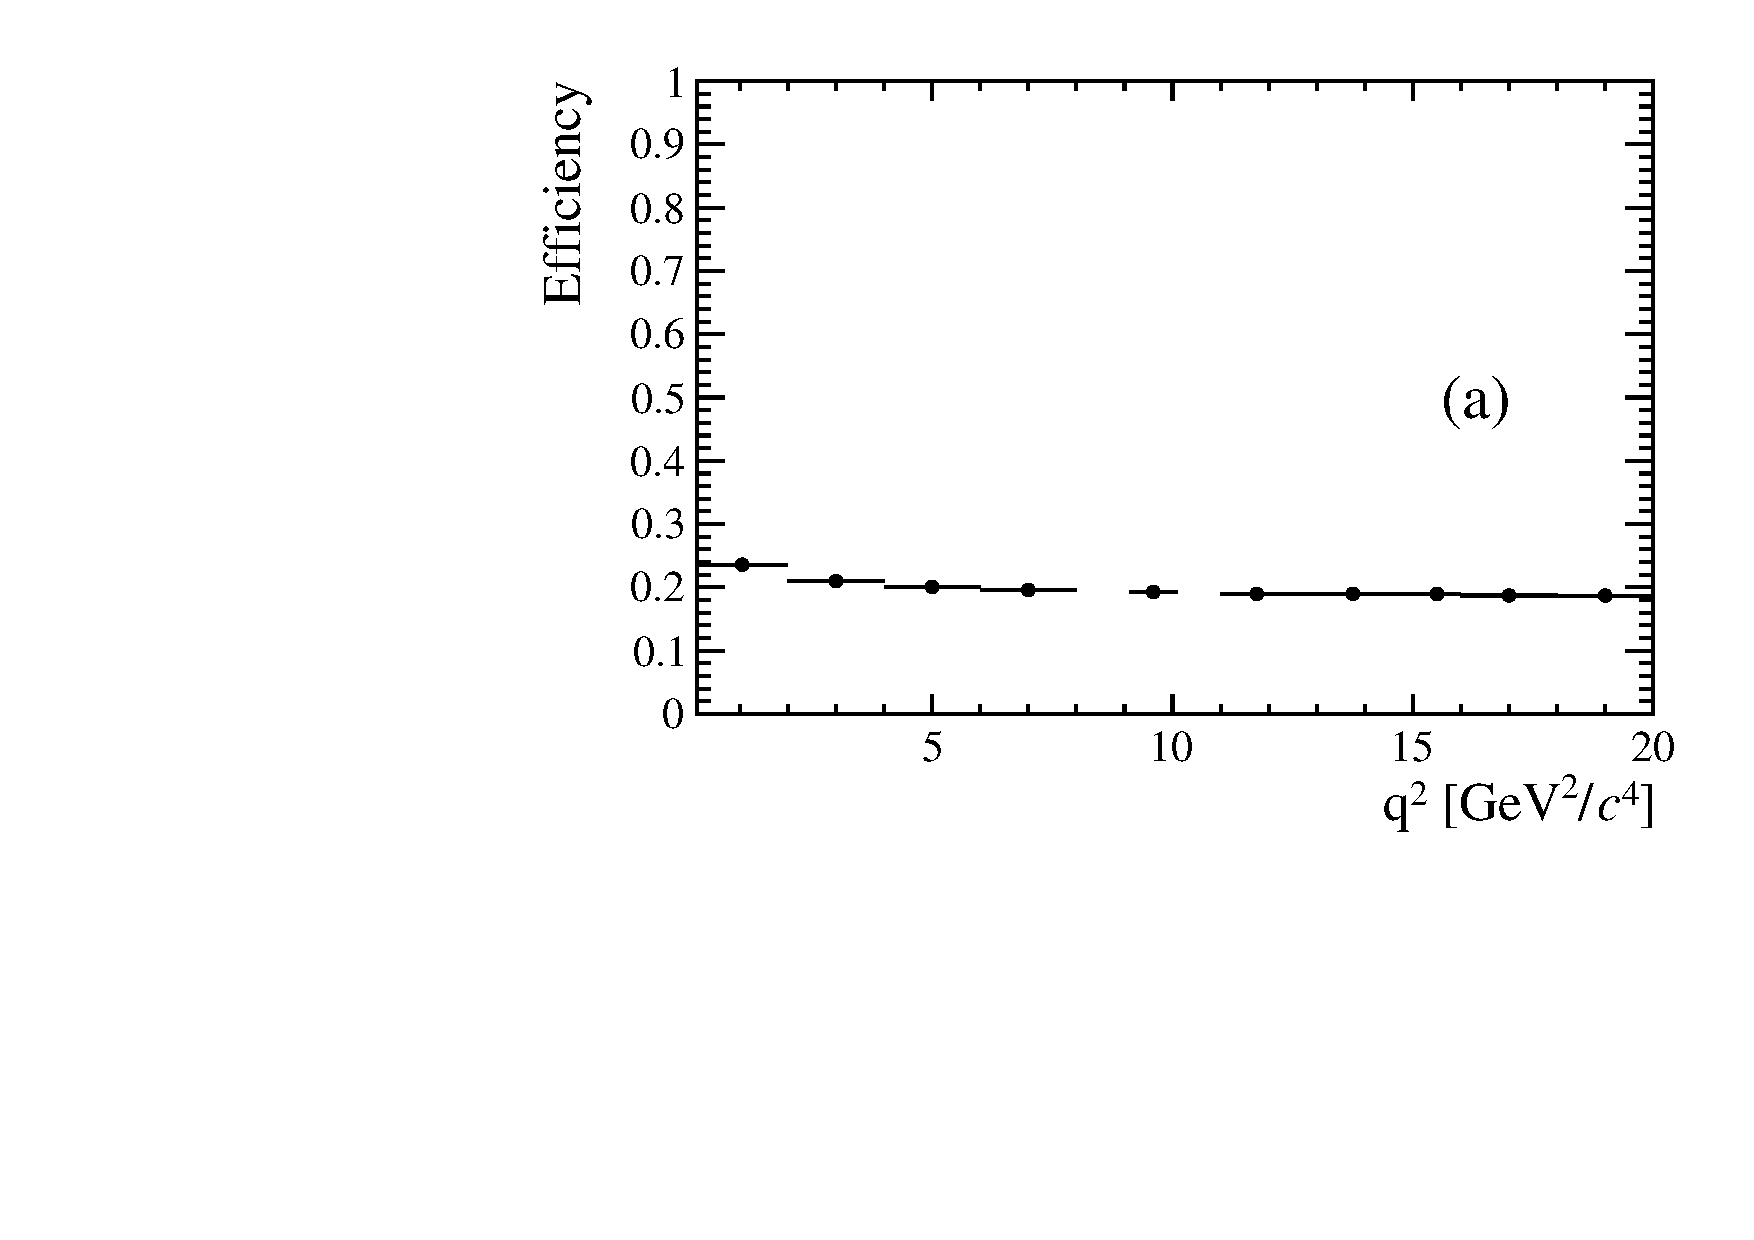
\includegraphics[width=0.49\textwidth]{Lmumu/figs/efficiencies/BR/effvsq2_DD_geom.pdf}
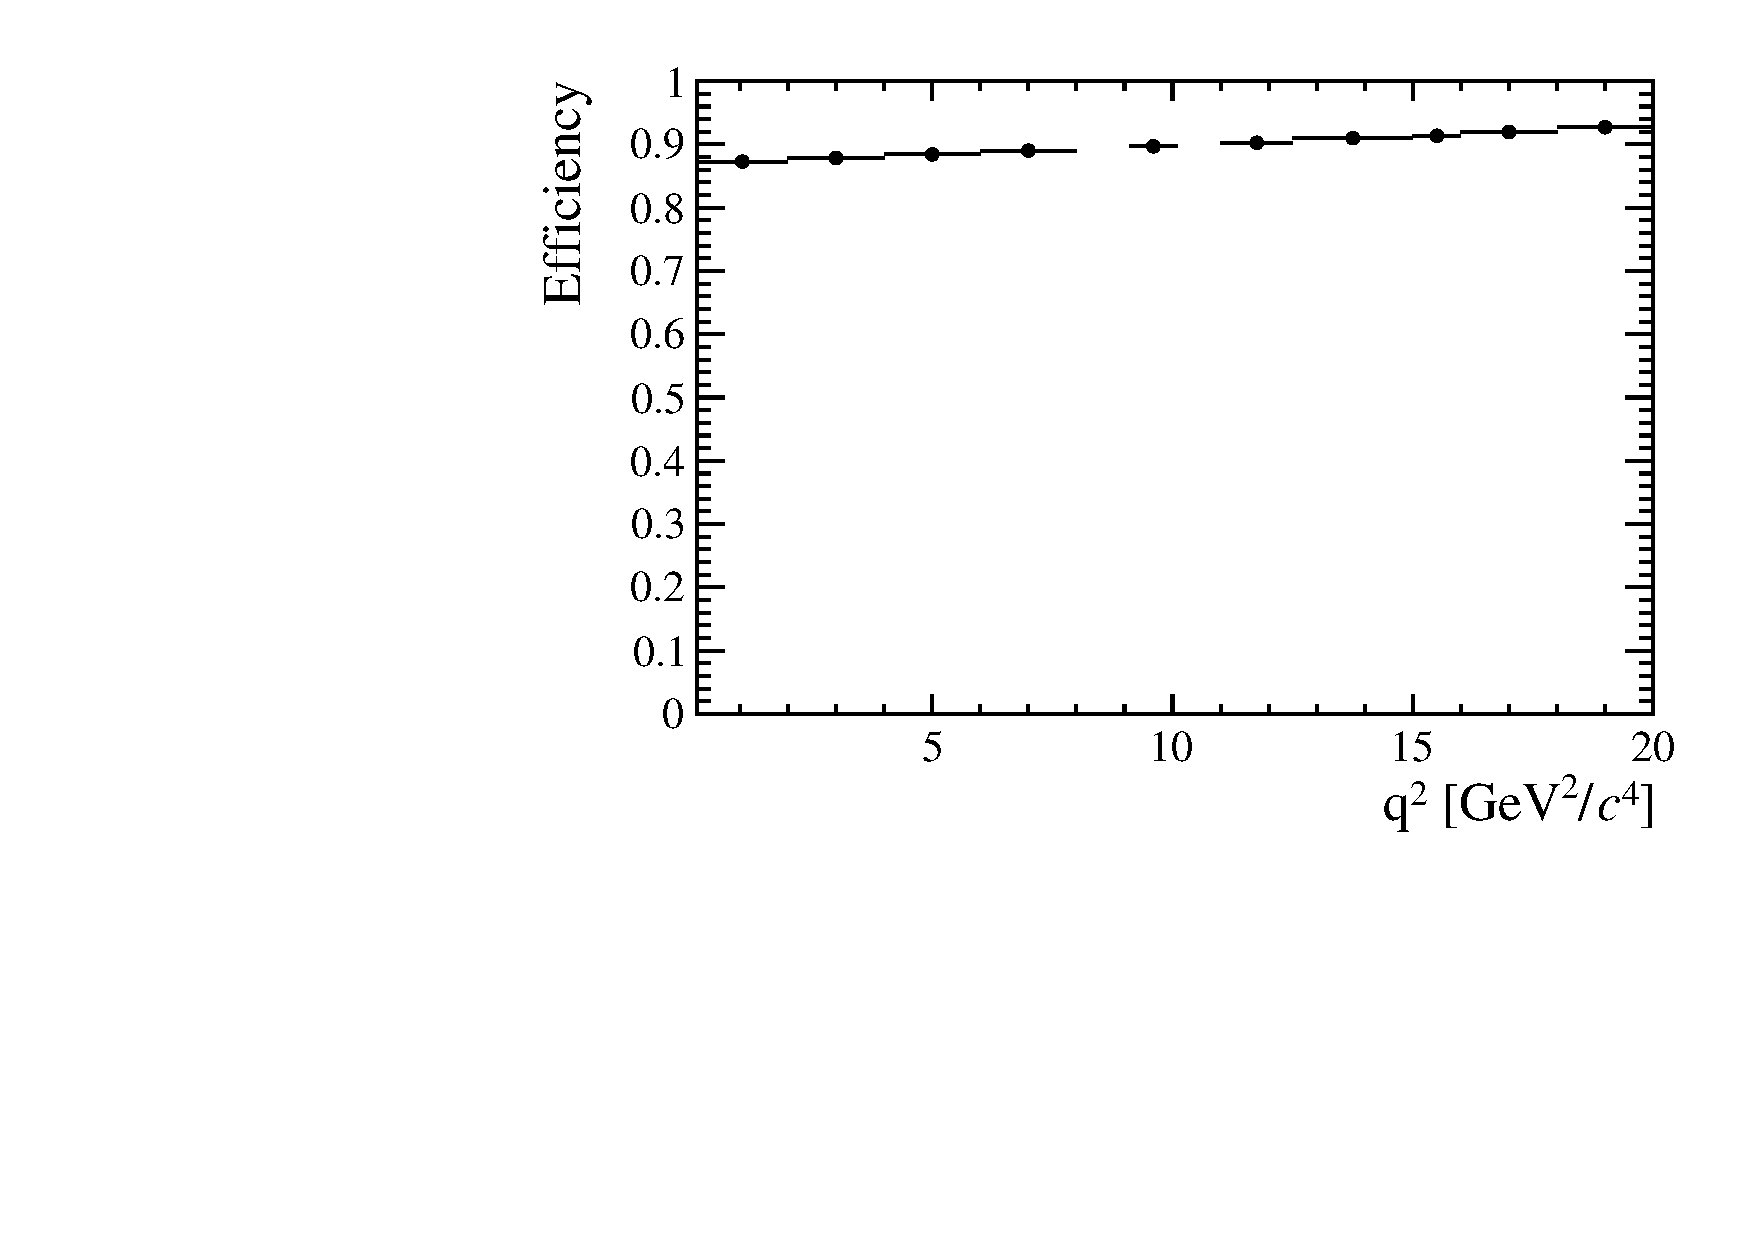
\includegraphics[width=0.49\textwidth]{Lmumu/figs/efficiencies/BR/effvsq2_DD_det.pdf}
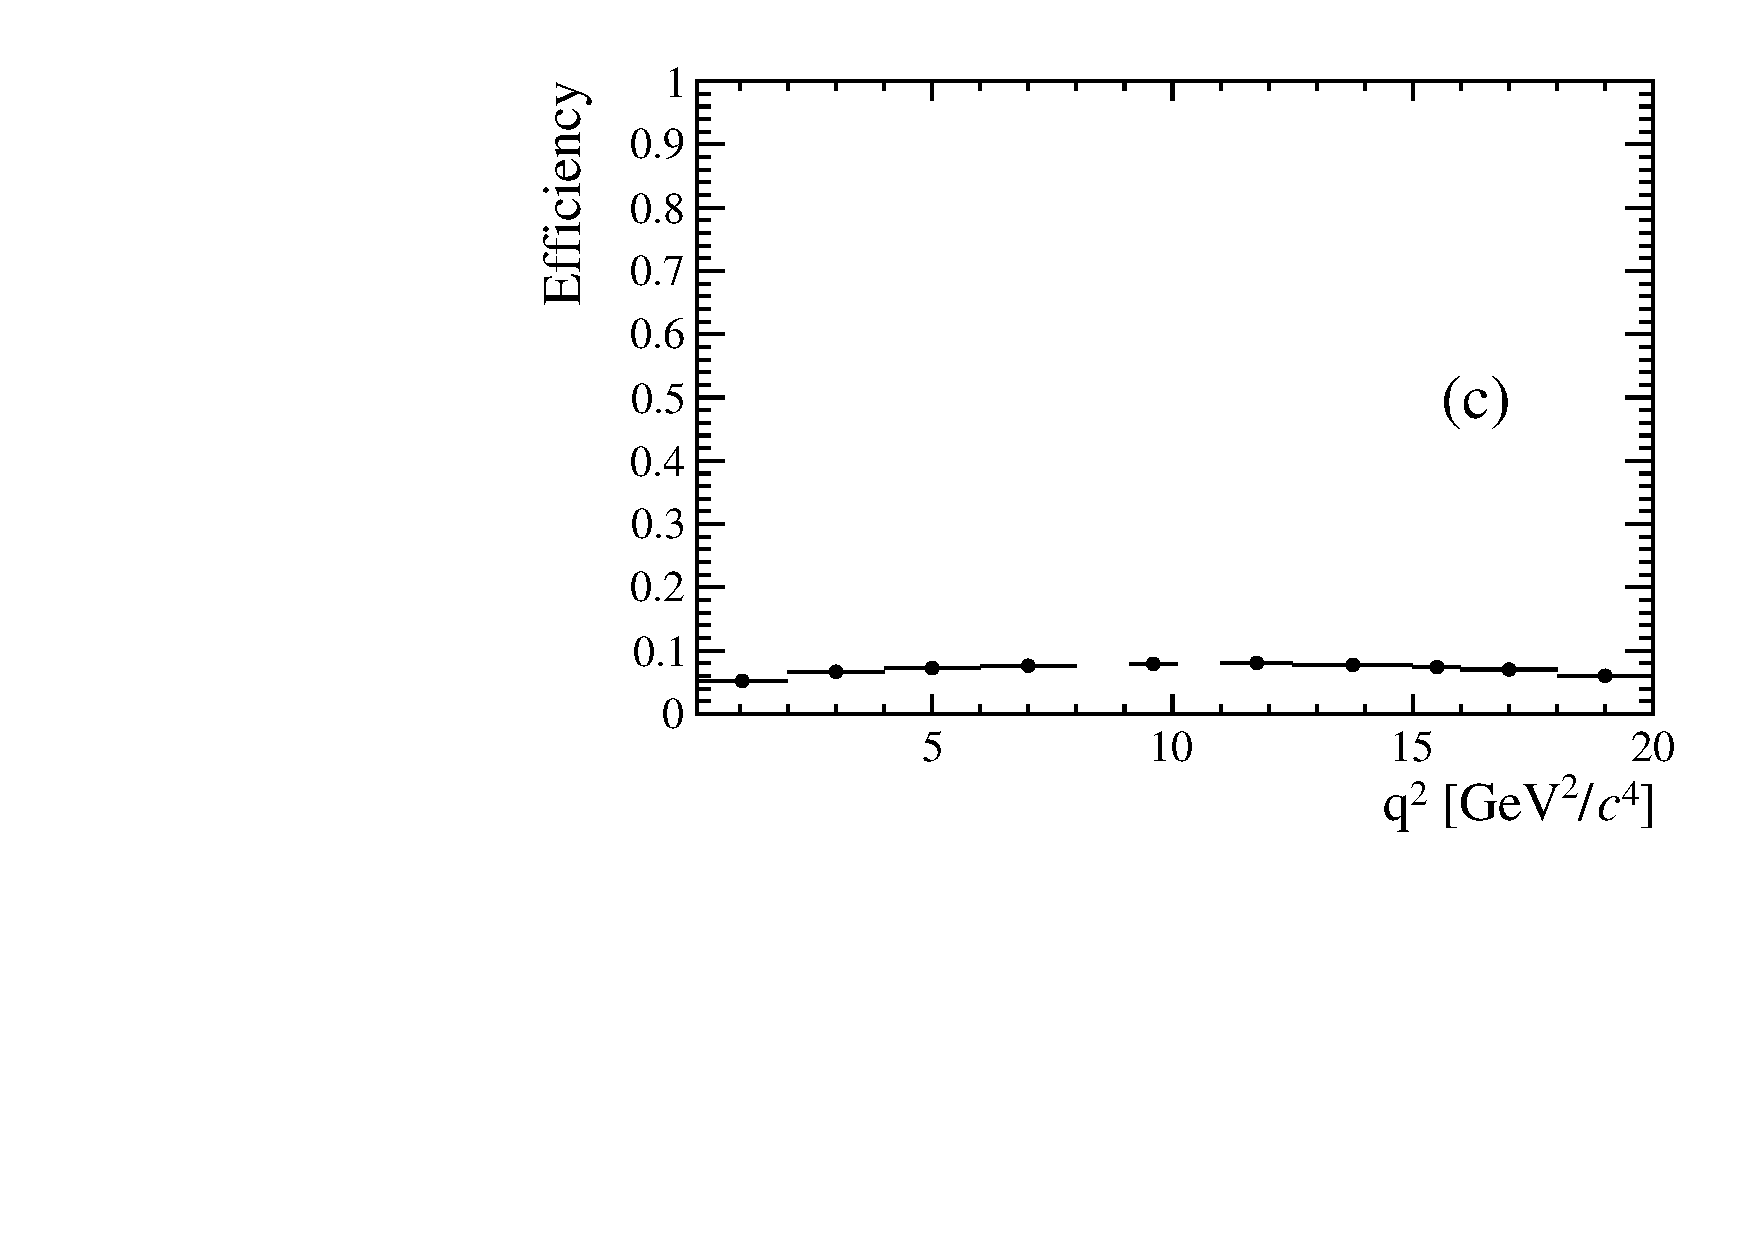
\includegraphics[width=0.49\textwidth]{Lmumu/figs/efficiencies/BR/effvsq2_DD_reco.pdf}
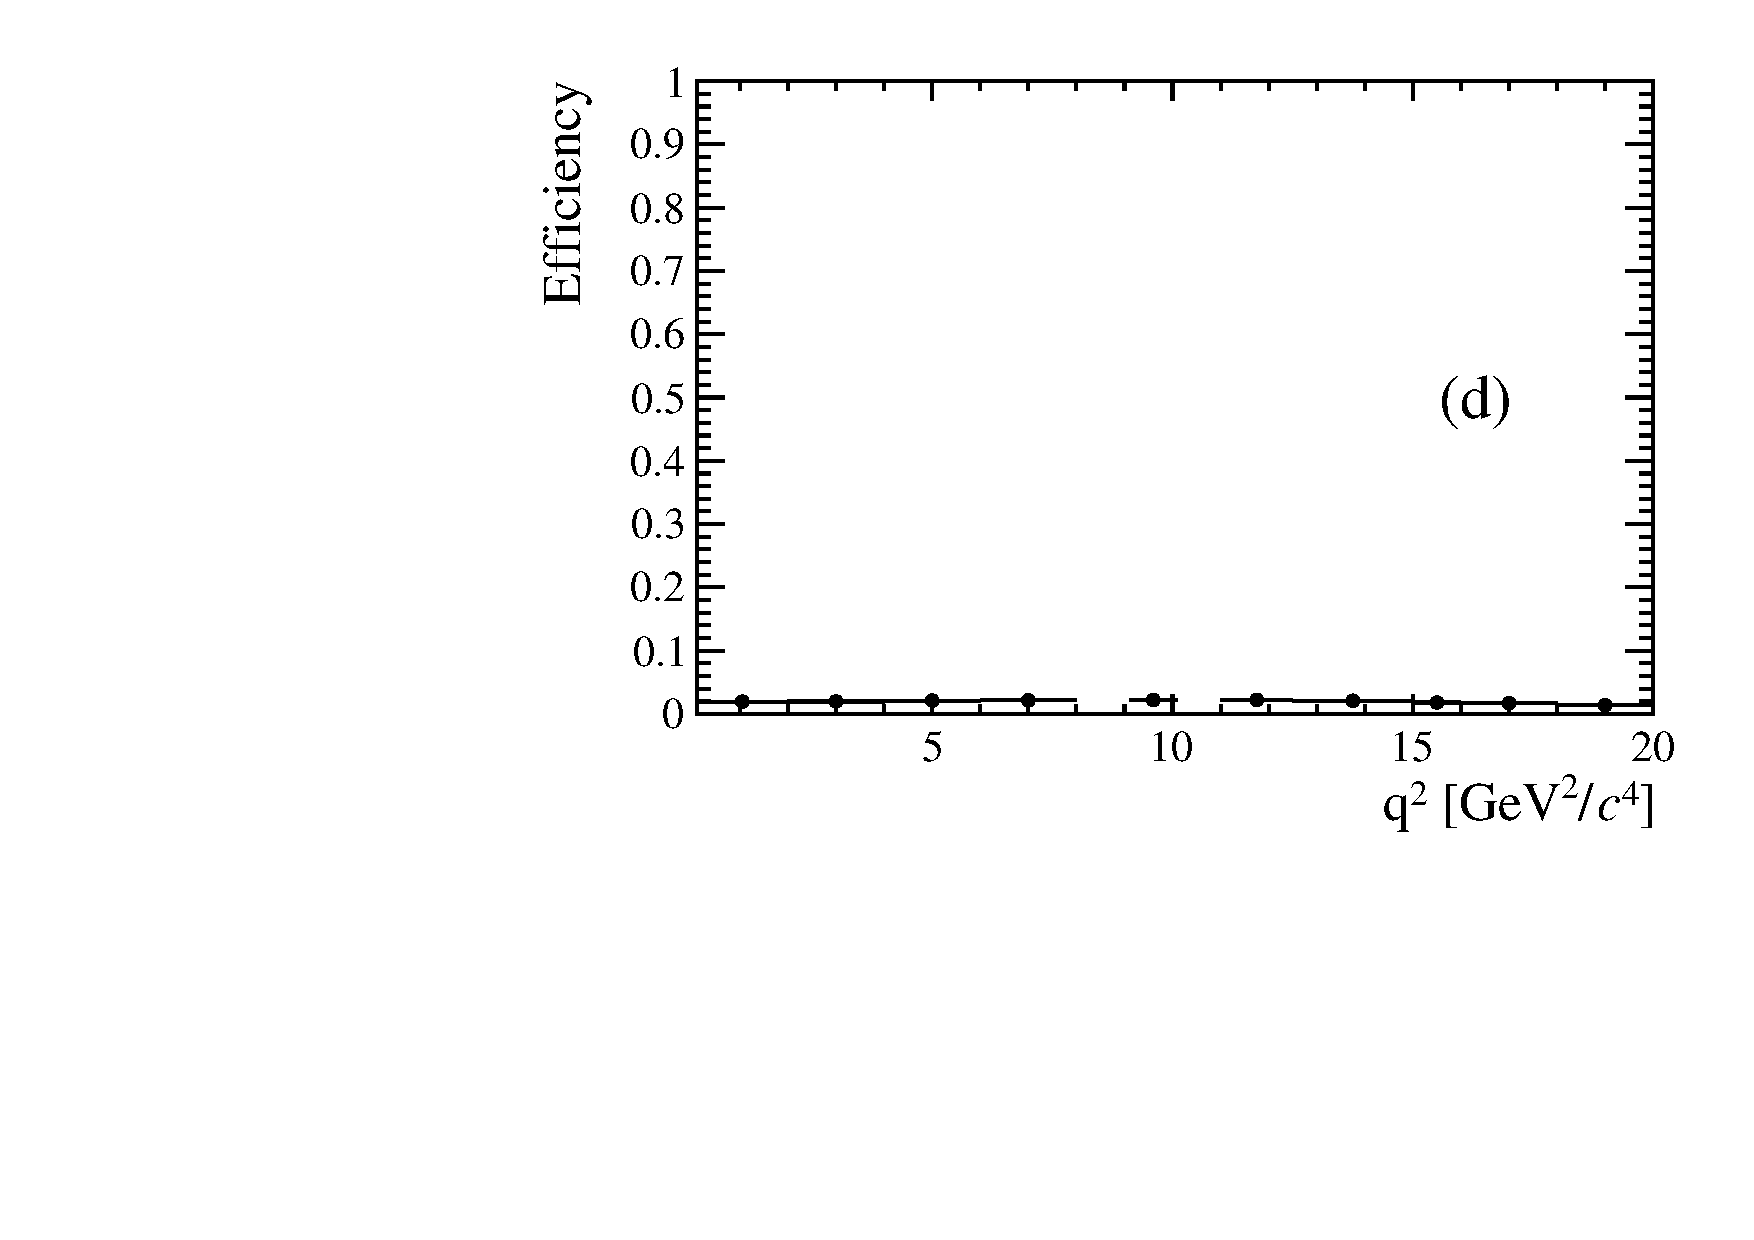
\includegraphics[width=0.49\textwidth]{Lmumu/figs/efficiencies/BR/effvsq2_LL_reco.pdf}
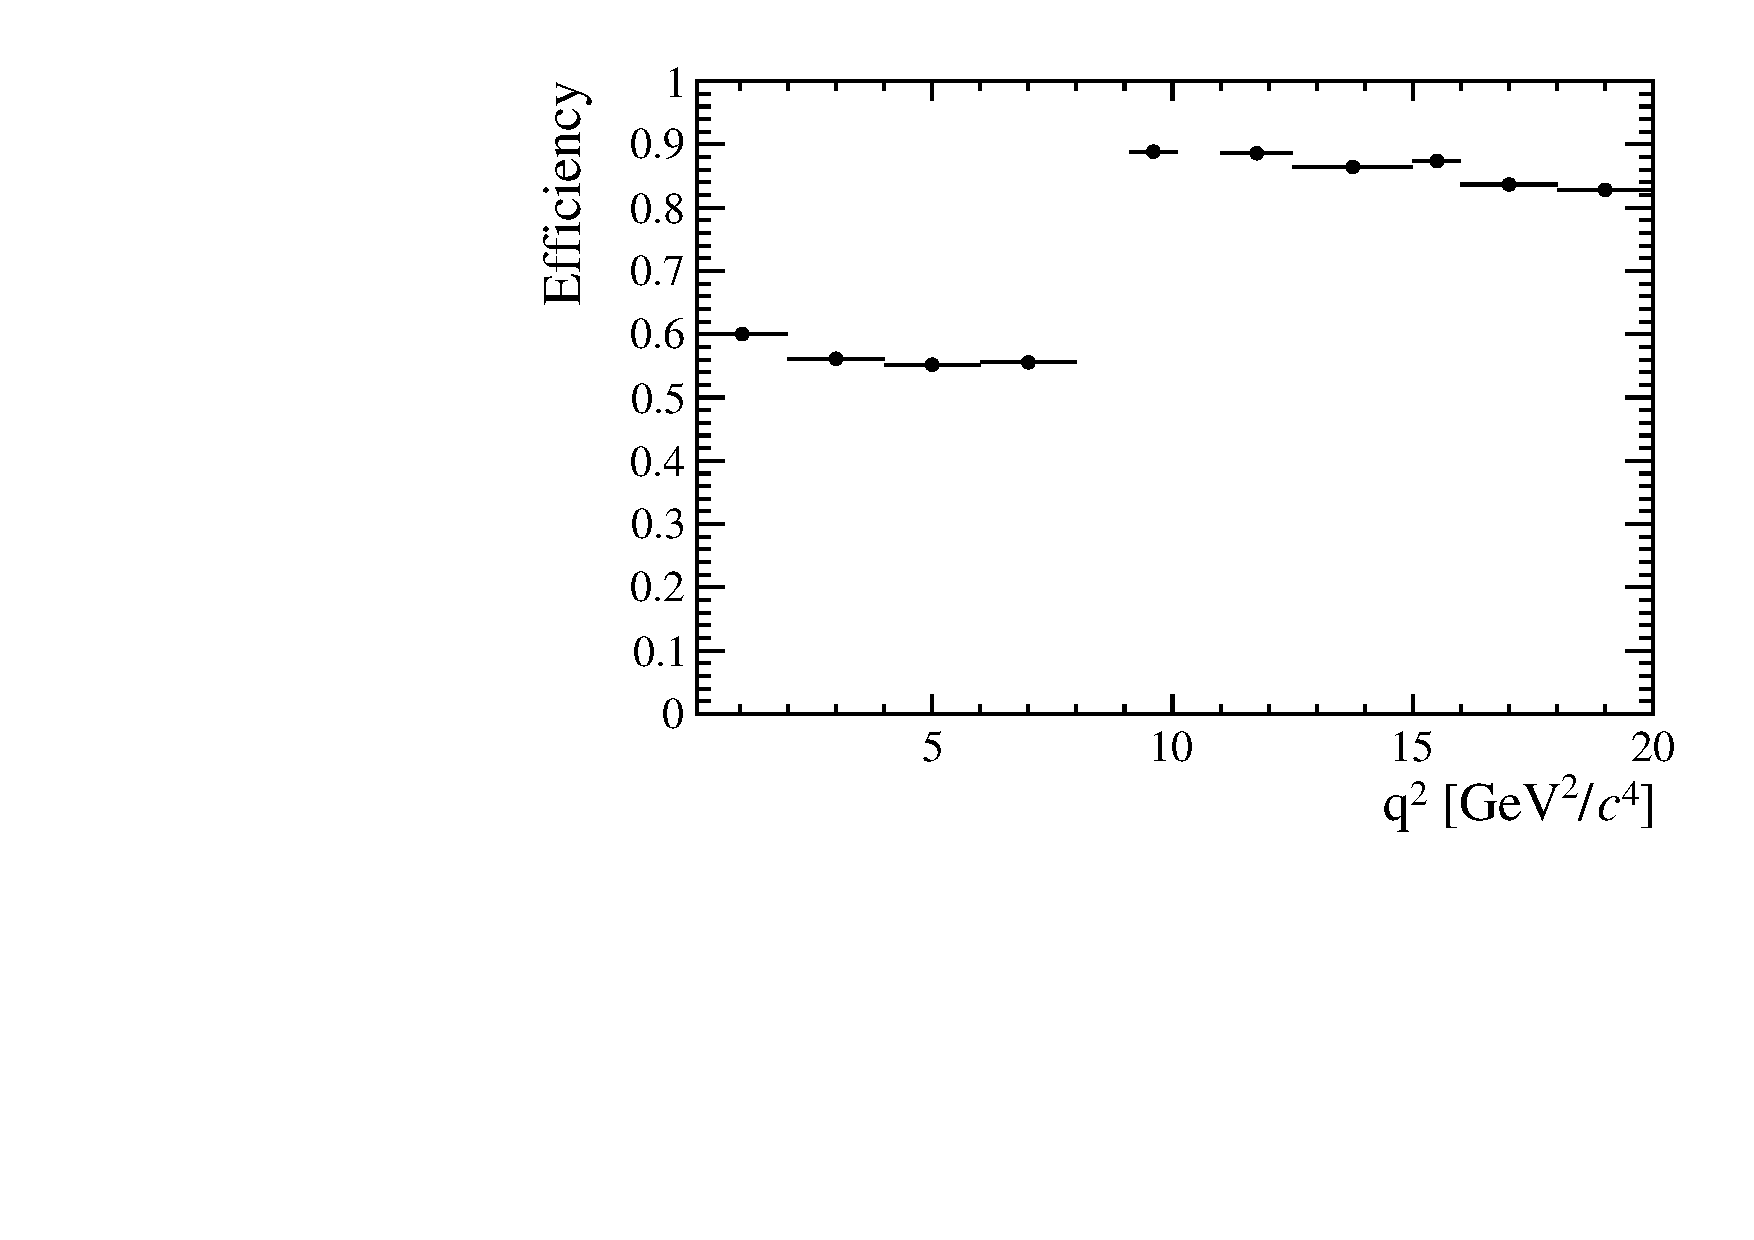
\includegraphics[width=0.49\textwidth]{Lmumu/figs/efficiencies/BR/effvsq2_DD_mva.pdf}
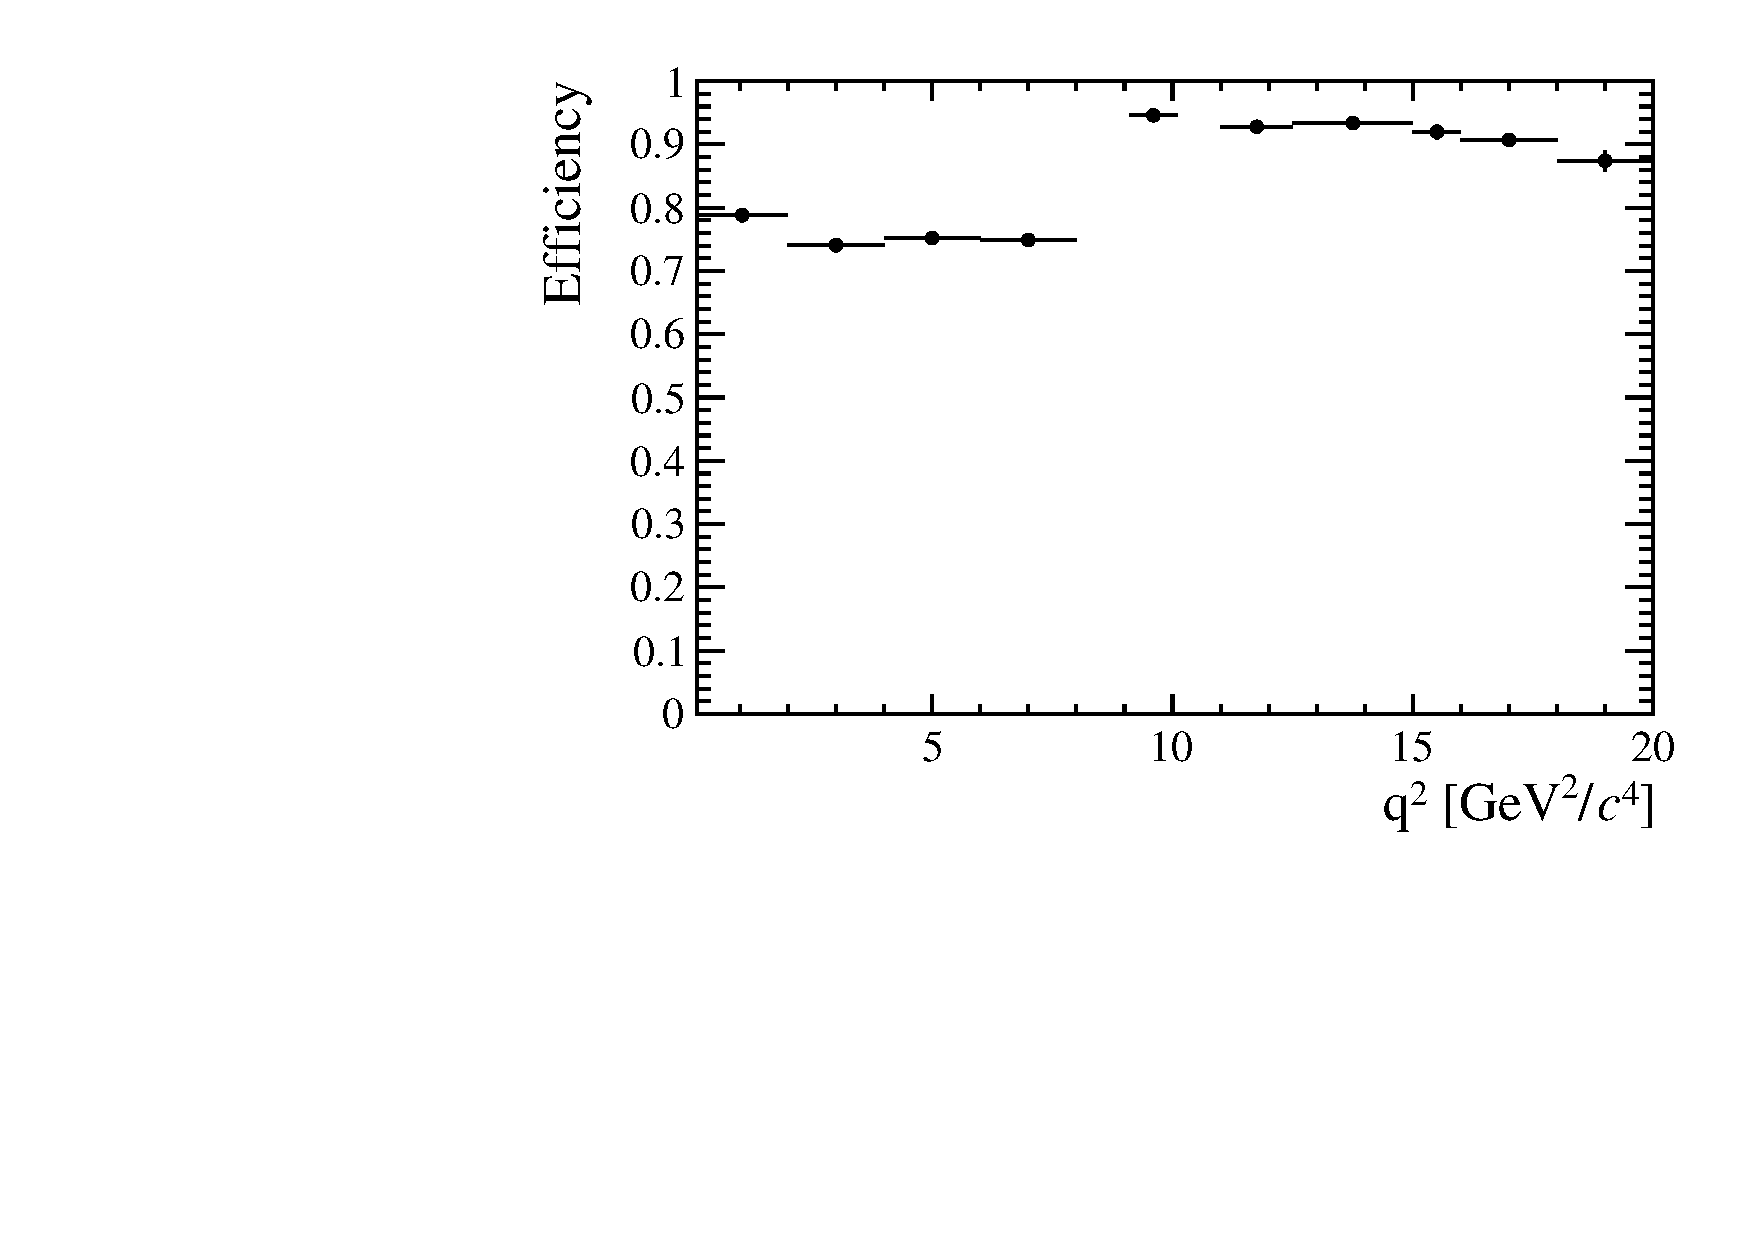
\includegraphics[width=0.49\textwidth]{Lmumu/figs/efficiencies/BR/effvsq2_LL_mva.pdf}
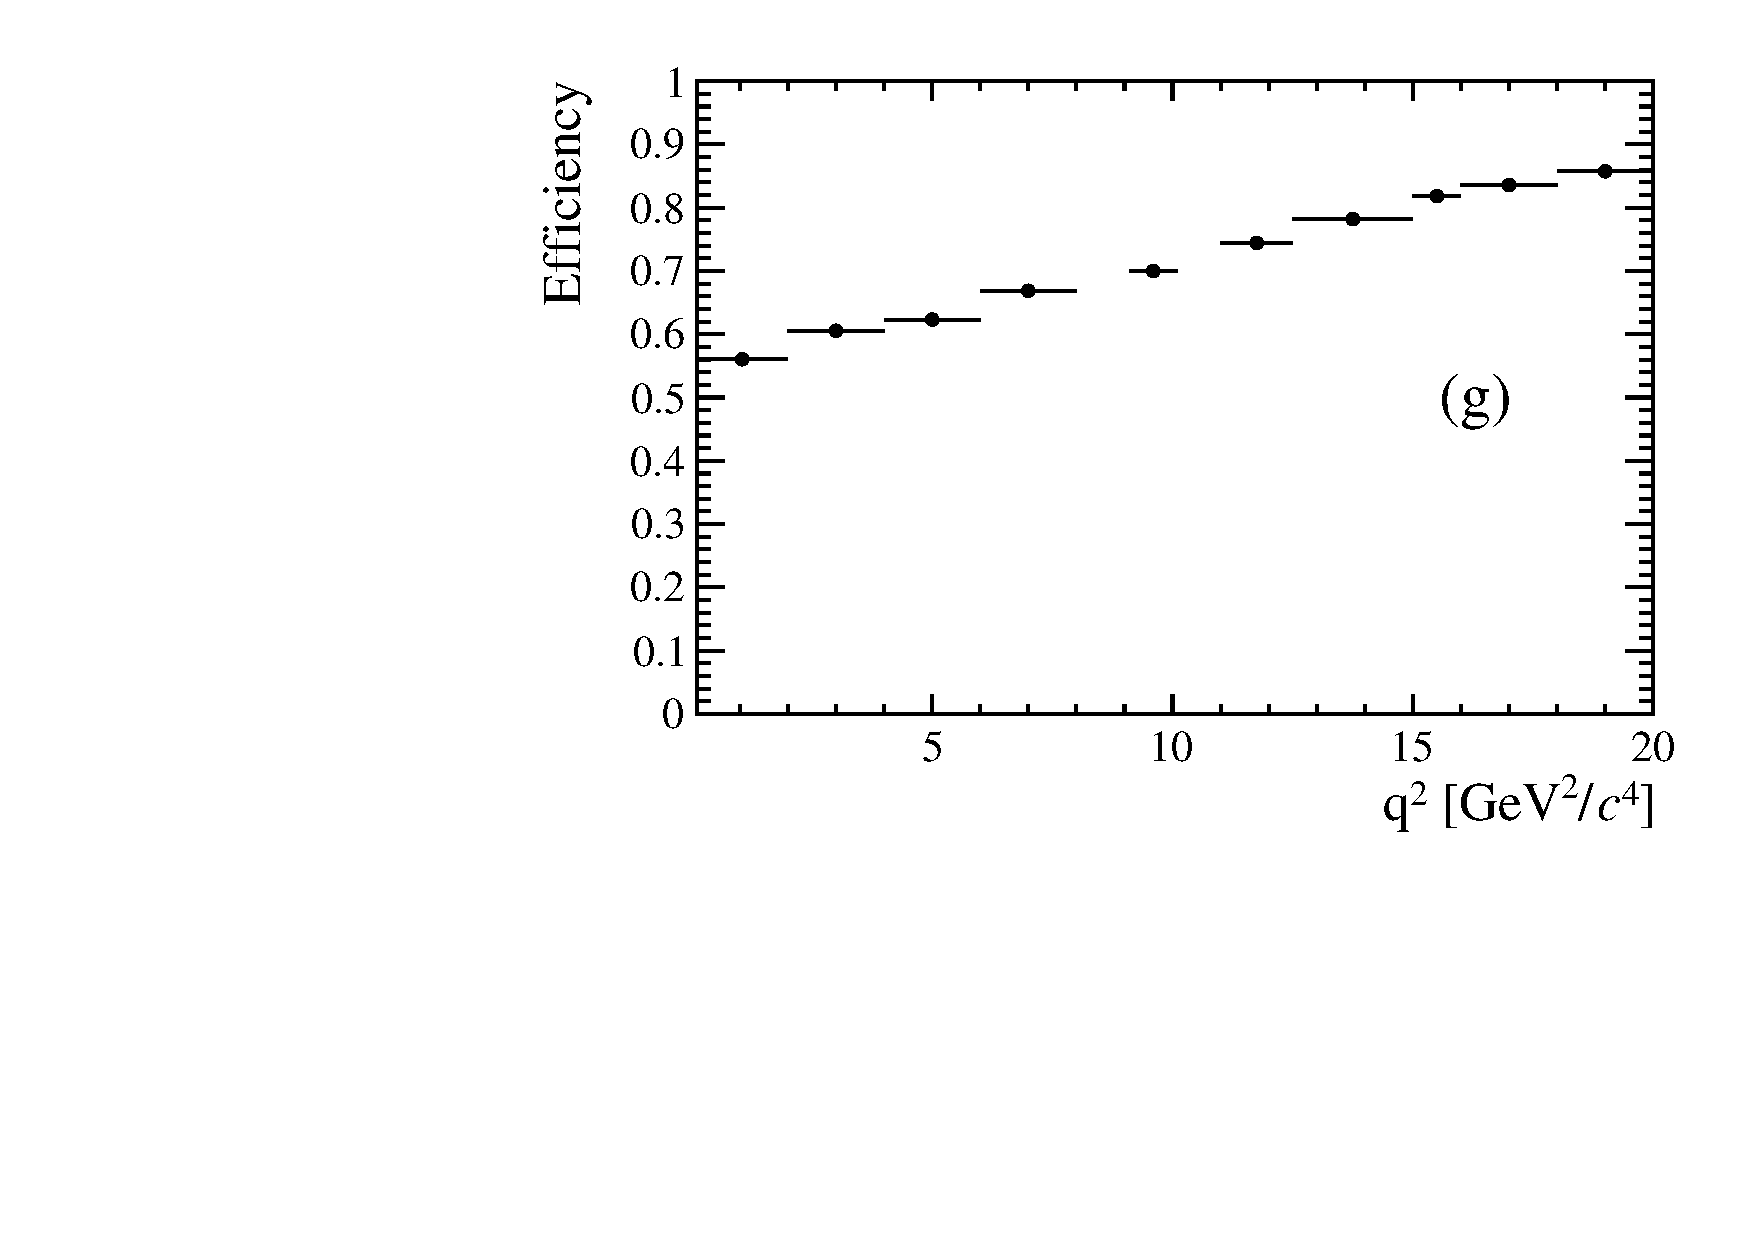
\includegraphics[width=0.49\textwidth]{Lmumu/figs/efficiencies/BR/effvsq2_DD_trig.pdf}
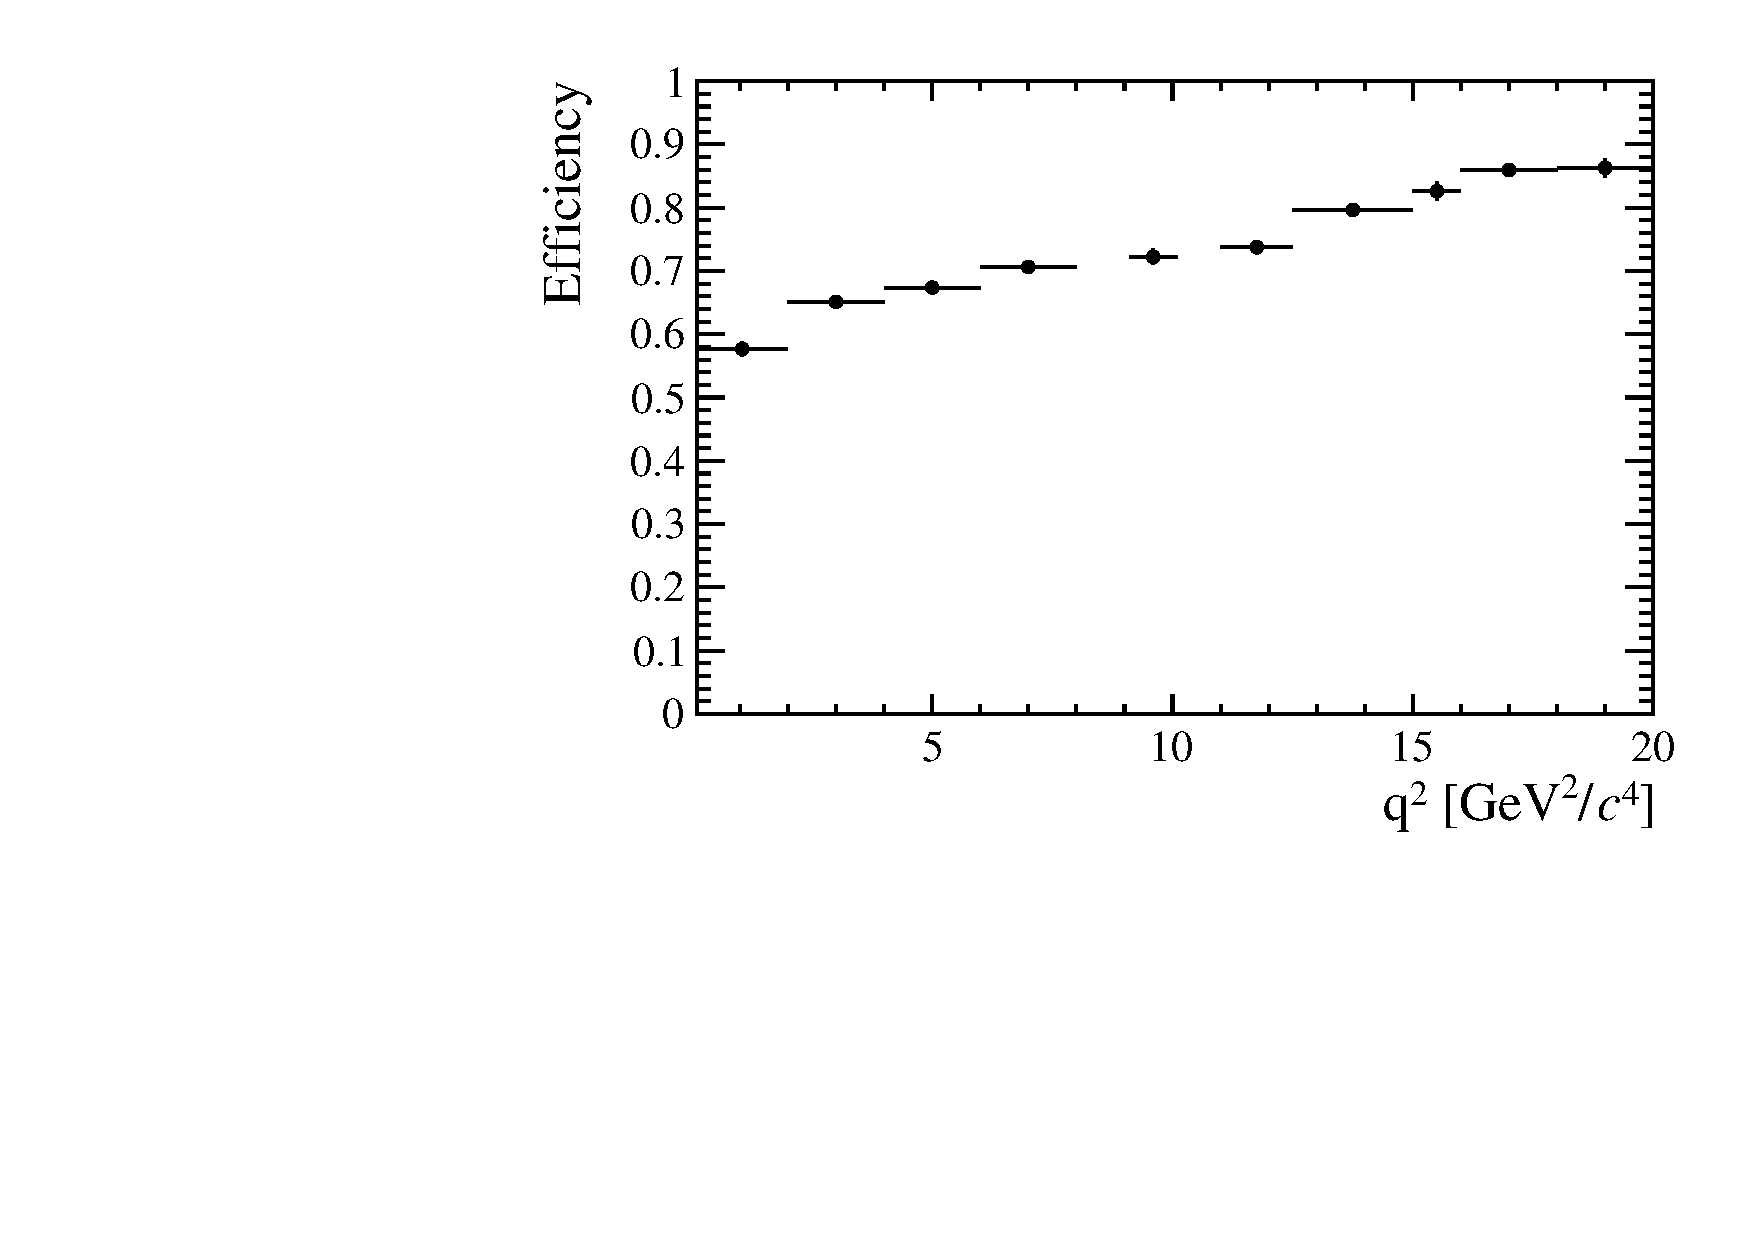
\includegraphics[width=0.49\textwidth]{Lmumu/figs/efficiencies/BR/effvsq2_LL_trig.pdf}
\caption{Absolute efficiencies as a function of \qsq: geometric efficiency (a); 
detection efficiency (b); reconstruction efficiency for DD (c) and LL (d) candidates; 
MVA efficiency for DD (e) and LL (f); trigger efficiency for DD (g) and LL (h).}
\label{fig:Lb_absEff}
\end{figure}

\clearpage
